% \section{Anexos}

% % === TEXTO ORIGINAL CORREGIDO ===
% Anexo 1: Diagrama de flujo

% % === FIGURA 2 ===
% \begin{figure}[H] % H mayúscula fuerza posición exacta
%     \centering
%     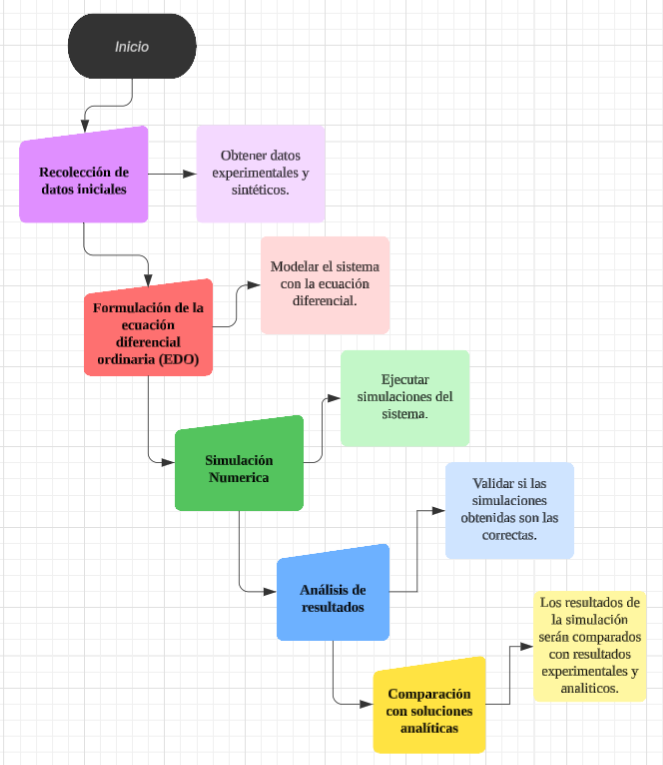
\includegraphics[width=0.8\textwidth]{5.png}
% \end{figure}
% Anexo 2: Código y gráfica de la carga en el capacitor vs. Tiempo

% % === FIGURA 3 ===
% \begin{figure}[h]
%     \centering
%     % añadir aca
% \end{figure}
\section{Anexos}
\vspace*{2cm}
Anexo 1: Diagrama de flujo
\begin{figure}[H]
    \centering
    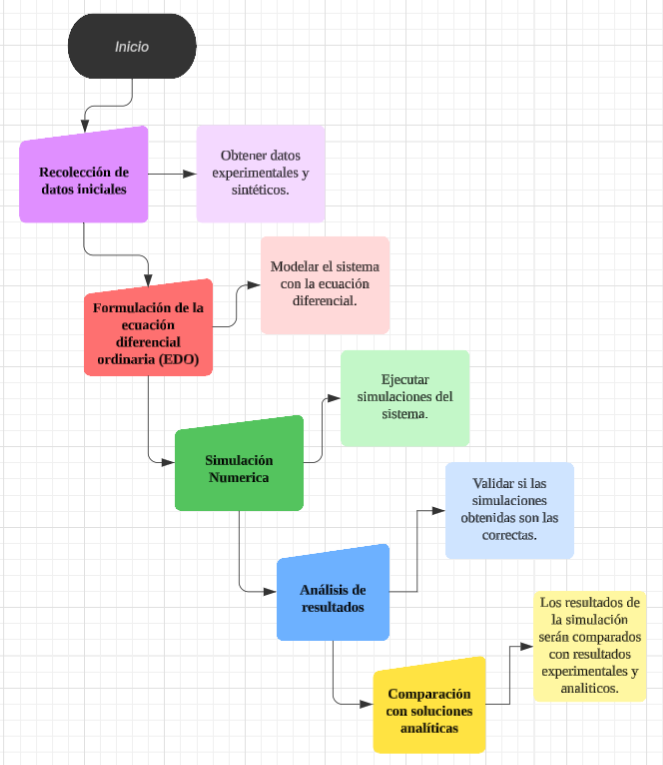
\includegraphics[width=0.8\textwidth]{5.png}
\end{figure}
\newpage
Anexo 2: Código y gráfica de la carga en el capacitor vs. Tiempo

\begin{figure}[H]
    \centering
    % Espacio para tu imagen (reemplaza "grafica_carga.png" con tu archivo)
    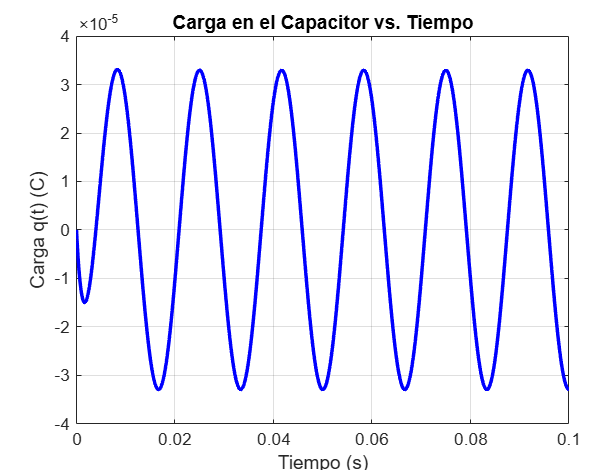
\includegraphics[width=0.8\textwidth]{6.png}
    \caption{Gráfica generada por el código MATLAB}
\end{figure}

% Cuadro con el código MATLAB
\begin{lstlisting}[language=Matlab, caption={Código MATLAB para simulación de carga}, label={cod:matlab}, frame=single, basicstyle=\footnotesize\ttfamily]
tau = 1.6e-3;        % Constante de tiempo
omega = 2 * pi * 60; % Frecuencia angular (60 Hz)
B = 5.4679e-8;       % Coeficiente B
C_p = -3.2982e-5;    % Coeficiente C_p
q = @(t) 3.2982e-5 * exp(-t / tau) + B * sin(omega * t) + C_p * cos(omega * t);
% Crear un rango de tiempo
t = linspace(0, 0.1, 1000); % Rango de 0 a 0.1 segundos
% Calcular q(t) para cada valor de t
q_t = q(t);
% Graficar q(t)
figure;
plot(t, q_t, 'b', 'LineWidth', 2);
title('Carga en el Capacitor vs. Tiempo');
xlabel('Tiempo (s)');
ylabel('Carga q(t) (C)');
grid on;
\end{lstlisting}